\documentclass[10pt]{beamer}

%\usepackage[utf8x]{inputenc}
%\usepackage[english]{babel}
\usepackage{beamerthemesplit}
\usepackage{amsmath}
\usepackage{graphicx}
\usetheme{Pittsburgh}
\usepackage{amssymb}
\usepackage{amsmath}
\usepackage{tabularx}

\title[Learning and optimizing using Gaussian Processes]{Three contributions to the design and analysis of computer models using Gaussian processes}
\author[V. Picheny]{\textcolor{blue}{Victor Picheny}\\
in collaboration with D. Ginsbourger, Y. Richet, G. Caplin, O. Roustant, N-H. Kim, R. Haftka}
\date{November 16th, 2012}

\AtBeginSection[]
{
\begin{frame}{Table of Contents}
	\tableofcontents[currentsection]
\end{frame}
}

\begin{document}

\frame{\titlepage}



%%%%%%%%%%%%%%%%%%%%%%%%%%%%%%%%%%%%%%%%%%%%%%%%%%%%%%%%%%%%%%%%%%%%%%%%%%%%%%%%%%%%%%%%%%%%%%%%
% \section{Introduction}
\frame
{
\frametitle{Introduction (1/2)}
\begin{block}{Context}
\begin{itemize}
 \item Numerical black-box experiments
 \item Moderate input dimension ($d \leq 50$), scalar output
 \item Continuous input / output spaces
\end{itemize}
\end{block}

 \begin{figure}[h!] \centering	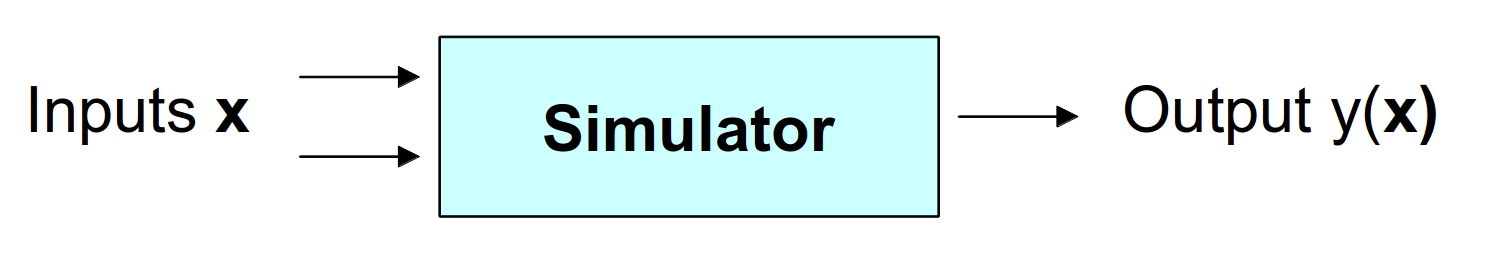
\includegraphics[width=8cm]{fig/simulator.png} \end{figure}

\begin{block}{Objectives}
Learning / optimization / inversion / reliability analysis / Sensitivity analysis
\end{block}

\begin{block}{Main issue}
Number of runs is very limited
\end{block}
}

%%%%%%%%%%%%%%%%%%%%%%%%%%%%%%%%%%%%%%%%%%%%%%%%%%%%%%%%%%%%%%%%%%%%%%%%%%%%%%%%%%%%%%%%%%%%%%%%
% \section{Introduction}
\frame
{
\frametitle{Introduction (2/2)}
\begin{block}{Popular solution: use of meta-models}
% \begin{itemize}
%  \item Experimental design $\mathbf{x}_1, \ldots, \mathbf{x}_n$
%  \item Set of measurements $y(\mathbf{x}_1), \ldots, y(\mathbf{x}_n)$
% \end{itemize}
\end{block}
\vspace{-5mm}
\begin{figure}[h!] \centering	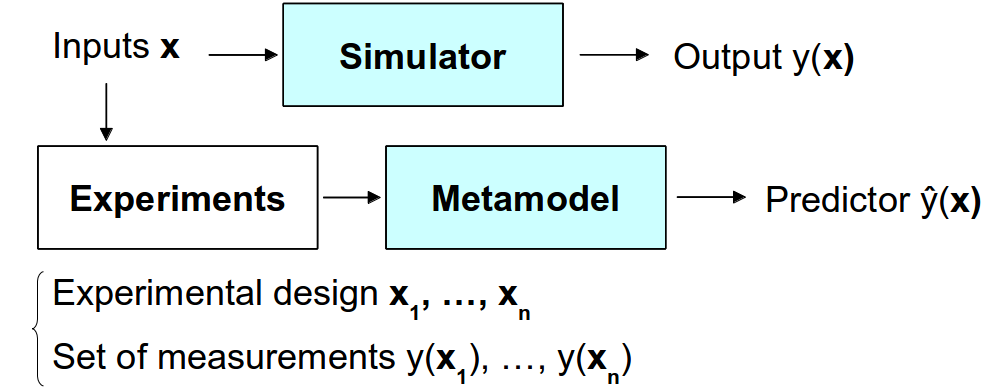
\includegraphics[width=9cm]{fig/metamodel.png} \end{figure}
\vspace{-4mm}
\begin{block}{Questions}
\vspace{-2mm}
\begin{itemize}
 \item How do we choose $\mathbf{x}_1, \ldots, \mathbf{x}_n$ (\textit{design of experiments})
 \item How do we build an accurate model (\textit{modeling})
 \item How do we use the model to pilot new experiments (\textit{sequential strategies})
\end{itemize}
\end{block}
}

%%%%%%%%%%%%%%%%%%%%%%%%%%%%%%%%%%%%%%%%%%%%%%%%%%%%%%%%%%%%%%%%%%%%%%%%%%%%%%%%%%%%%%%%%%%%%%%%%
\frame{
\frametitle{Outline}
\tableofcontents
}

%%%%%%%%%%%%%%%%%%%%%%%%%%%%%%%%%%%%%%%%%%%%%%%%%%%%%%%%%%%%%%%%%%%%%%%%%%%%%%%%%%%%%%%%%%%%%%%%%
%%%%%%%%%%%%%%%%%%%%%%%%%%%%%%%%%%%%%%%%%%%%%%%%%%%%%%%%%%%%%%%%%%%%%%%%%%%%%%%%%%%%%%%%%%%%%%%%%
\section{Basics of Gaussian Process modeling}
%%%%%%%%%%%%%%%%%%%%%%%%%%%%%%%%%%%%%%%%%%%%%%%%%%%%%%%%%%%%%%%%%%%%%%%%%%%%%%%%%%%%%%%%%%%%%%%%%
%%%%%%%%%%%%%%%%%%%%%%%%%%%%%%%%%%%%%%%%%%%%%%%%%%%%%%%%%%%%%%%%%%%%%%%%%%%%%%%%%%%%%%%%%%%%%%%%%

%%%%%%%%%%%%%%%%%%%%%%%%%%%%%%%%%%%%%%%%%%%%%%%%%%%%%%%%%%%%%%%%%%%%%%%%%%%%%%%%%%%%%%%%%%%%%%%%%%
\frame{\frametitle{Introduction to Gaussian process regression 1/4} Actual function (output vs. input) \begin{figure}[h!] \centering	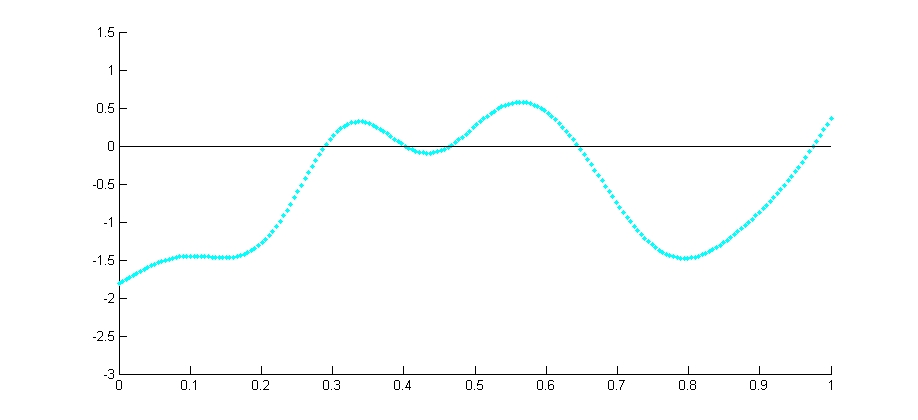
\includegraphics[width=10cm]{fig/f1.png} \end{figure} }
%%%%%%%%%%%%%%%%%%%%%%%%%%%%%%%%%%%%%%%%%%%%%%%%%%%%%%%%%%%%%%%%%%%%%%%%%%%%%%%%%%%%%%%%%%%%%%%%%%
\frame{\frametitle{Introduction to Gaussian process regression 2/4} What we have: experimental design \begin{figure}[h!]  \centering	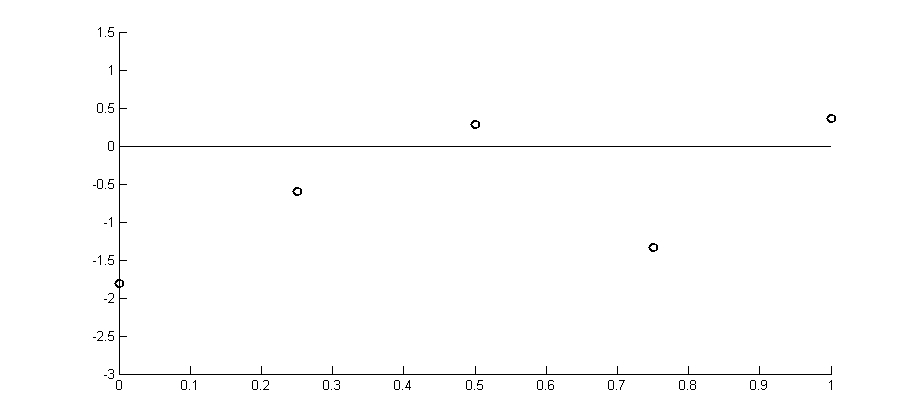
\includegraphics[width=10cm]{fig/f2.png} \end{figure} }
%%%%%%%%%%%%%%%%%%%%%%%%%%%%%%%%%%%%%%%%%%%%%%%%%%%%%%%%%%%%%%%%%%%%%%%%%%%%%%%%%%%%%%%%%%%%%%%%%%
\frame{\frametitle{Introduction to Gaussian process regression 3/4} Possible paths,conditional on the data (assumptions needed!) \begin{figure}[h!]  \centering	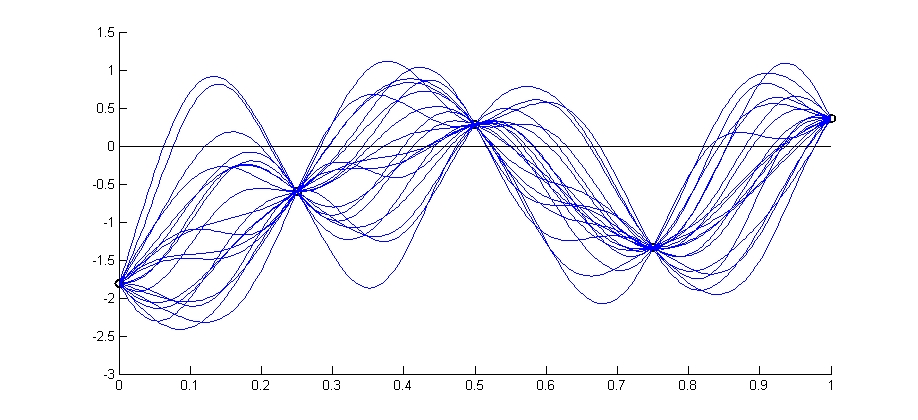
\includegraphics[width=10cm]{fig/f3.png} \end{figure} }
%%%%%%%%%%%%%%%%%%%%%%%%%%%%%%%%%%%%%%%%%%%%%%%%%%%%%%%%%%%%%%%%%%%%%%%%%%%%%%%%%%%%%%%%%%%%%%%%%
\frame{\frametitle{Introduction to Gaussian process regression 4/4} GP model: mean and variance \begin{figure}[h!]  \centering	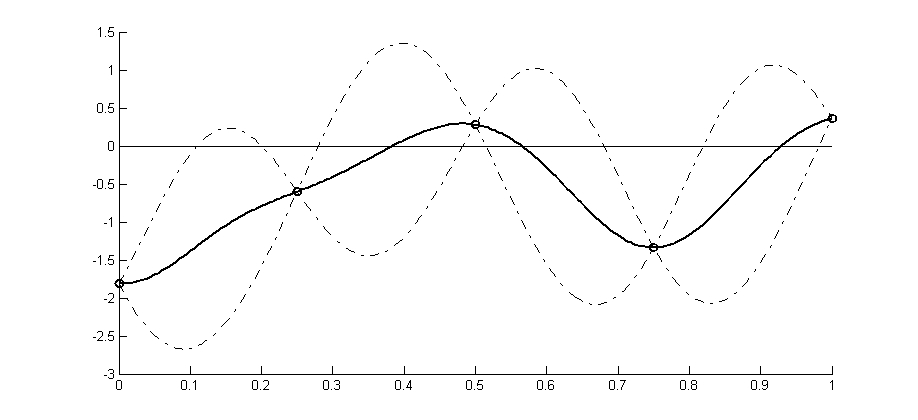
\includegraphics[width=10cm]{fig/f4.png} \end{figure} }
%%%%%%%%%%%%%%%%%%%%%%%%%%%%%%%%%%%%%%%%%%%%%%%%%%%%%%%%%%%%%%%%%%%%%%%%%%%%%%%%%%%%%%%%%%%%%%%%%%

%%%%%%%%%%%%%%%%%%%%%%%%%%%%%%%%%%%%%%%%%%%%%%%%%%%%%%%%%%%%%%%%%%%%%%%%%%%%%%%%%%%%%%%%%%%%%%%%
\frame
{
\frametitle{A little bit of theory (1/2)}
\begin{block}{Assumption}
$y$ is one path of a Gaussian Process $\left(Y_{\mathbf{x}}\right)_{\mathbf{x} \in D}$ with known covariance
$k$ and trend $\mu(x) =\sum_{i=0}^p \beta_i f_i(\mathbf{x})$ known up to the linear coefficients $\beta_i \in \mathbb{R}$
\end{block}

\begin{block}{The covariance function}
\begin{itemize}
 \item (Usually) stationary: $cov \left( Y_{\mathbf{x}_1}, Y_{\mathbf{x}_2} \right) = k(\mathbf{x}_2 - \mathbf{x}_1)$
 \item Defines the model characteristics: smoothness, regularity, amplitude...
 \item Requires a complex learning step (likelihood, cross-validation, ...)
\end{itemize}
\end{block}
}

%%%%%%%%%%%%%%%%%%%%%%%%%%%%%%%%%%%%%%%%%%%%%%%%%%%%%%%%%%%%%%%%%%%%%%%%%%%%%%%%%%%%%%%%%%%%%%%%
\frame
{
\frametitle{A little bit of theory (2/2)}

\begin{block}{Kriging Equations}
Simply Gaussian process conditioning
\begin{itemize}
 \item Conditional expectation: $m_{krig}(\mathbf{x}^*) = m \left(\mathbf{x}^* | y(\mathbf{x}_1), \ldots, y(\mathbf{x}_n) \right)$
 \item Conditional variance (or covariance): $c_{krig}(\mathbf{x}^*,\mathbf{x}^{**}) = cov(\mathbf{x}^*, \mathbf{x}^{**}| y(\mathbf{x}_1), \ldots, y(\mathbf{x}_n) )$
\end{itemize}
\end{block}

\begin{block}{\textit{Probabilistic} metamodel}
\begin{itemize}
 \item Associates a \textbf{distribution} to a set of prediction points \\
 \item In particular, for each point: a \textbf{best predictor} $m_{krig}(\mathbf{x}^*)$ (response surface) and a \textbf{prediction error variance} $s_{krig}^2(\mathbf{x}^*) = c_{krig}(\mathbf{x}^*,\mathbf{x}^{*})$
\end{itemize}
$\rightarrow$ Rich information for the user!
\end{block}
}

%%%%%%%%%%%%%%%%%%%%%%%%%%%%%%%%%%%%%%%%%%%%%%%%%%%%%%%%%%%%%%%%%%%%%%%%%%%%%%%%%%%%%%%%%%%%%%%%
\section{Adaptive designs for accurate critical regions approximation}
%%%%%%%%%%%%%%%%%%%%%%%%%%%%%%%%%%%%%%%%%%%%%%%%%%%%%%%%%%%%%%%%%%%%%%%%%%%%%%%%%%%%%%%%%%%%%%%%

\frame
{
\frametitle{Motivation}

\begin{block}{Global versus ``targeted'' learning}
\begin{itemize}
 \item Sampling strategy has a strong effect on local accuracy
 \item Accuracy is not needed everywhere!
\end{itemize}
\end{block}

\begin{figure}[h!] \centering	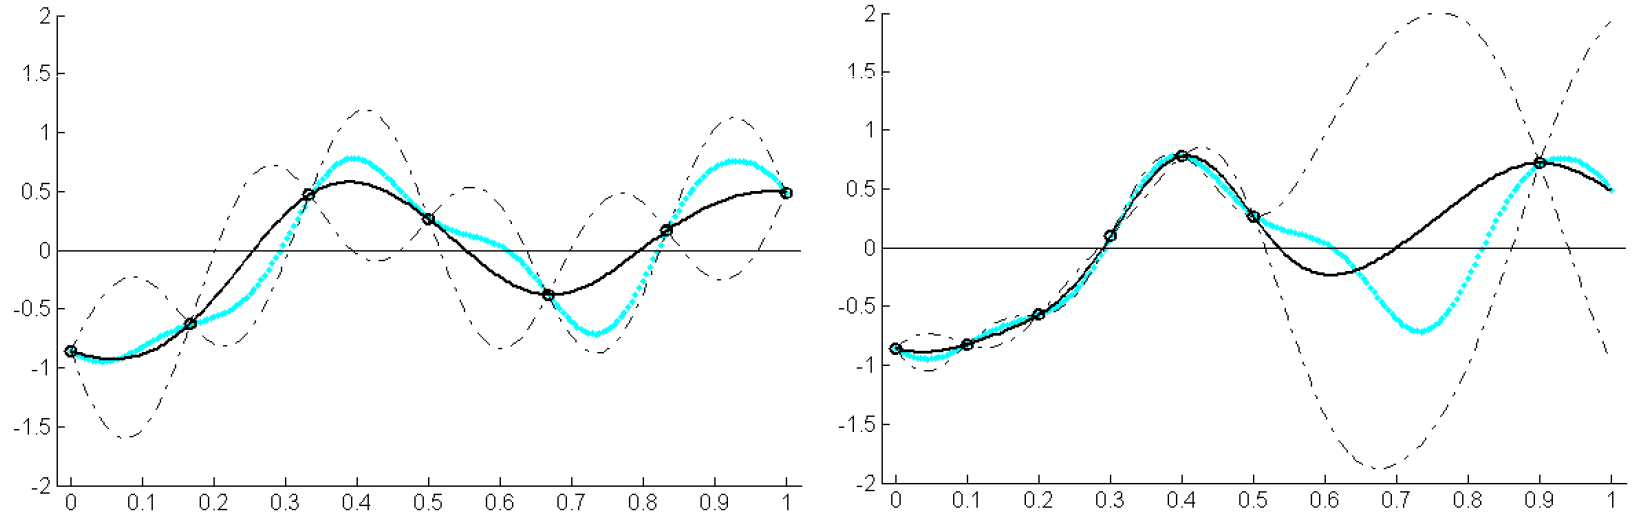
\includegraphics[width=10cm]{fig/two7pointskrigs.png} \end{figure}
}

%%%%%%%%%%%%%%%%%%%%%%%%%%%%%%%%%%%%%%%%%%%%%%%%%%%%%%%%%%%%%%%%%%%%%%%%%%%%%%%%%%%%%%%%%%%%%%%%
\frame
{
\frametitle{The problem considered}

\begin{block}{\textit{Level sets} critical regions}
\begin{itemize}
 \item Risk management: we want to know if $y(\mathbf{x}) \geq T$
 \item Applications: probability of failure, constrained optimization...
  \item $y(\mathbf{x}) \ll T$ or $y(\mathbf{x}) \gg T$: inaccurate model is sufficient
 \item Critical region (for learning): $X_T = \left\{ \mathbf{x} / y(\mathbf{x}) \approx T \right\}$
\end{itemize}
\end{block}

\begin{block}{Objective}
\begin{itemize}
 \item Kriging model accurate in critical regions
 \item Sequential sampling $\rightarrow$ criterion for choosing measurements one by one
\end{itemize}
\end{block}
}

%%%%%%%%%%%%%%%%%%%%%%%%%%%%%%%%%%%%%%%%%%%%%%%%%%%%%%%%%%%%%%%%%%%%%%%%%%%%%%%%%%%%%%%%%%%%%%%%
\frame
{
\frametitle{Optimal designs for kriging}
\begin{columns}[t]
\begin{column}{6cm}
\begin{block}{Classical criterion: Integrated Mean Square Error (IMSE)}
\begin{itemize}
 \item Average prediction variance:
 \begin{eqnarray}
  IMSE &=& \int_D var(Y(\mathbf{x}) | \mathbf{Y}_n) d\mu(\mathbf{x}) \nonumber \\
       &=& \int_D s_{krig}^2(\mathbf{x}) d\mu(\mathbf{x}) \nonumber
  \end{eqnarray}
 
  \item Global measure of accuracy
 \item Does not depend on measurement values!
\end{itemize}
\end{block}

\end{column}

\begin{column}{6cm}
\begin{figure}
	\centering
		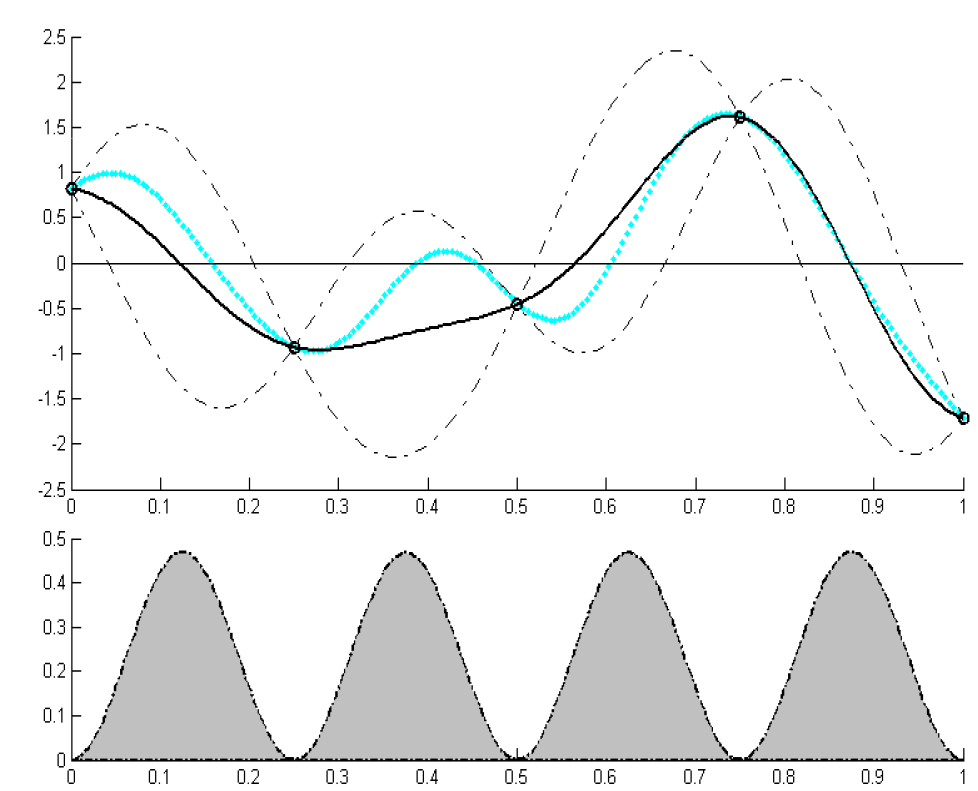
\includegraphics[width=5cm]{fig/IMSE.png}
\end{figure}	

\end{column}
\end{columns}
}

%%%%%%%%%%%%%%%%%%%%%%%%%%%%%%%%%%%%%%%%%%%%%%%%%%%%%%%%%%%%%%%%%%%%%%%%%%%%%%%%%%%%%%%%%%%%%%%%
\frame
{
\frametitle{Adapting IMSE for target learning}
\begin{block}{Exploiting the model information}
\begin{itemize}
	\item Critical region: $X_T = \left\{ \mathbf{x} / \left| y(\mathbf{x}) - T  \right| \leq \varepsilon \right\}$
	\item We can compute analytically the conditional probability $P\left(\mathbf{x} \in X_T \right)$:
	$$P\left(\mathbf{x} \in X_T \right) = \Phi \left( \frac{T + \varepsilon - m_{krig}(\mathbf{x})}{s_{krig}(\mathbf{x})} \right) - \Phi \left( \frac{T - \varepsilon - m_{krig}(\mathbf{x})}{s_{krig}(\mathbf{x})} \right)$$
\end{itemize}
\end{block}

\begin{block}{New criterion}
Prediction variance weighted by the probability to belong to the target region:
$$IMSE_T = \int_D var(Y(\mathbf{x}) | \mathbf{Y}_n) P\left(\mathbf{x} \in X_T \right)d\mu(\mathbf{x})$$
Trade-off between global accuracy and exploration of target regions
\end{block}
}

%%%%%%%%%%%%%%%%%%%%%%%%%%%%%%%%%%%%%%%%%%%%%%%%%%%%%%%%%%%%%%%%%%%%%%%%%%%%%%%%%%%%%%%%%%%%%%%%
\frame
{
\frametitle{Illustration: modification of the integrand}
\begin{figure}
	\centering
		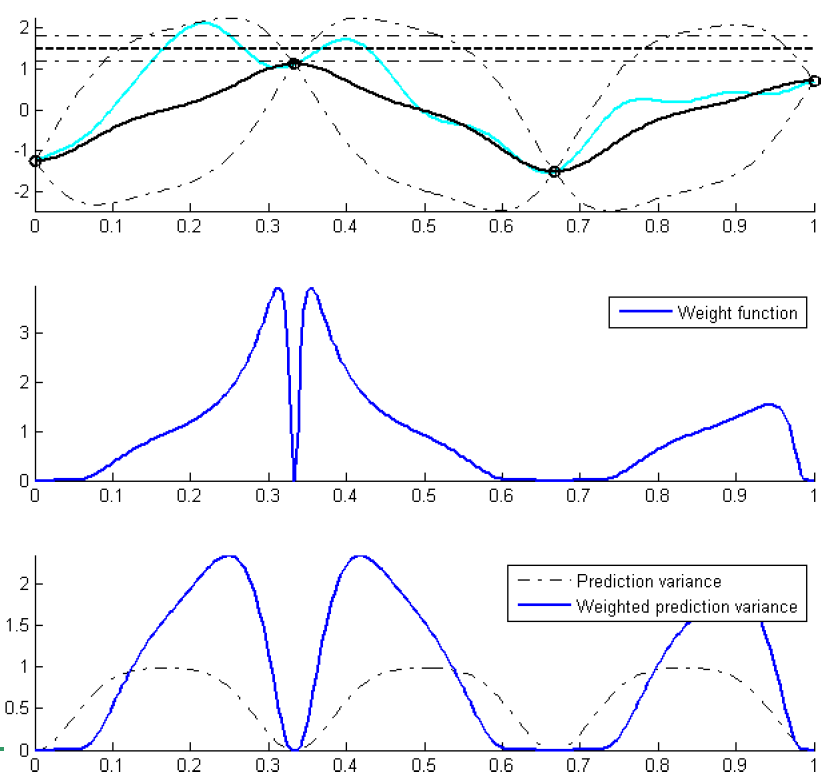
\includegraphics[width=60mm]{fig/illustIMSET.png}
\end{figure}	
}

%%%%%%%%%%%%%%%%%%%%%%%%%%%%%%%%%%%%%%%%%%%%%%%%%%%%%%%%%%%%%%%%%%%%%%%%%%%%%%%%%%%%%%%%%%%%%%%%
\frame
{
\frametitle{Adaptation to sequential sampling}
\begin{itemize}
 \item Measure of the effect of adding a measurement on the criterion:
$$IMSE_T(\mathbf{x}_{new}) = \int_D var(Y(\mathbf{x}) | \mathbf{Y}_n, \mathbf{x}_{new}) P\left(\mathbf{x} \in X_T \right)d\mu(\mathbf{x})$$
 \item At each $n$: $\mathbf{x}_{n+1} = \arg \max IMSE_T(\mathbf{x}_{new})$
\end{itemize}

\begin{figure}
	\centering
		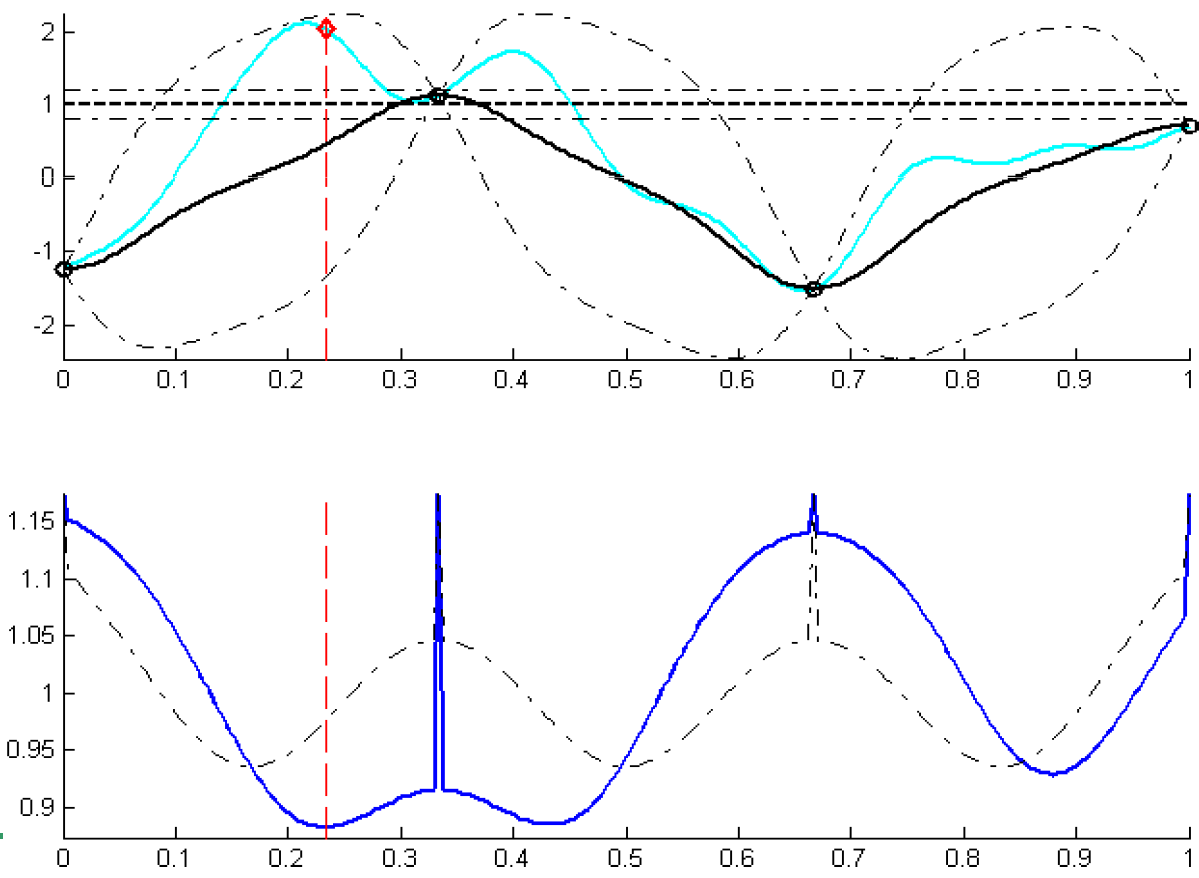
\includegraphics[width=60mm]{fig/illustIMSETseq.png}
\end{figure}	
}


%%%%%%%%%%%%%%%%%%%%%%%%%%%%%%%%%%%%%%%%%%%%%%%%%%%%%%%%%%%%%%%%%%%%%%%%%%%%%%%%%%%%%%%%%%%%%%%%
\frame
{
\frametitle{Illustration: 2 initial points + 7 iterations}
\begin{figure}
	\centering
		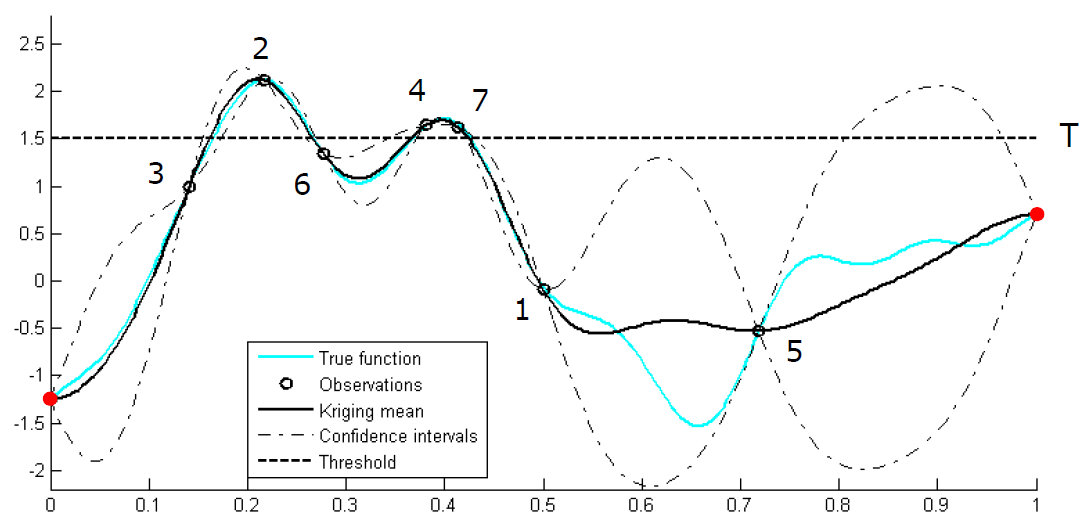
\includegraphics[width=85mm]{fig/illustOptIMSET.png}
\end{figure}	
}

%%%%%%%%%%%%%%%%%%%%%%%%%%%%%%%%%%%%%%%%%%%%%%%%%%%%%%%%%%%%%%%%%%%%%%%%%%%%%%%%%%%%%%%%%%%%%%%%
\frame
{
\frametitle{Some perspectives}
\begin{block}{Applications}
\begin{itemize}
	\item Problems addressed: probability of failure estimation, inversion
	\item Safety assessment of nuclear storage systems (with IRSN)
	\item Sensor deployment (with IRSN)
\end{itemize}
\end{block}

\begin{block}{Implementation}
R package \textit{KrigInv}
\end{block}

\begin{block}{On-going work}
\begin{itemize}
	\item Application to constrained optimization
	\item Application to quantile estimation
\end{itemize}
\end{block}
}

%%%%%%%%%%%%%%%%%%%%%%%%%%%%%%%%%%%%%%%%%%%%%%%%%%%%%%%%%%%%%%%%%%%%%%%%%%%%%%%%%%%%%%%%%%%%%%%%
\section{Optimization with noisy measurements}
%%%%%%%%%%%%%%%%%%%%%%%%%%%%%%%%%%%%%%%%%%%%%%%%%%%%%%%%%%%%%%%%%%%%%%%%%%%%%%%%%%%%%%%%%%%%%%%%

%%%%%%%%%%%%%%%%%%%%%%%%%%%%%%%%%%%%%%%%%%%%%%%%%%%%%%%%%%%%%%%%%%%%%%%%%%%%%%%%%%%%%%%%%%%%%%%%%
\frame
{
\frametitle{Optimization with kriging: state-of-the-art (1/2)}

\begin{block}{The optimization problem}
\vspace{-1mm}
\begin{itemize}
	\item Search for best set of input parameters: $\mathbf{x}^* = \arg \min_{\mathbf{x} \in D} y(\mathbf{x})$
	\item Box-constrained, continuous inputs 
\end{itemize}
\end{block}

\begin{block}{Objective: \textit{global} optimization}
\vspace{-1mm}
\begin{itemize}
	\item Balance between exploration and exploitation
	\item Parcimonious
	\item Derivate-free
\end{itemize}
\end{block}

\begin{block}{Model-based criterion for choosing observations}
\vspace{-1mm}
\begin{itemize}
	\item We take advantage of the uncertainty information of the model
	\item Balance between exploration and exploitation = balance between high kriging variance and low kriging mean
\end{itemize}
\end{block}
}

%%%%%%%%%%%%%%%%%%%%%%%%%%%%%%%%%%%%%%%%%%%%%%%%%%%%%%%%%%%%%%%%%%%%%%%%%%%%%%%%%%%%%%%%%%%%%%%%%
\frame
{
\frametitle{Optimization with kriging: state-of-the-art (1/2)}

\begin{block}{Model-based criterion for choosing observations}
\begin{itemize}
	\item We take advantage of the uncertainty information of the model
	\item Balance between exploration and exploitation = balance between high kriging variance and low kriging mean
\end{itemize}
\end{block}

\begin{block}{A very efficient solution: the EGO algorithm (Jones et al., 1998)}
\begin{itemize}
	\item Based on an \textit{indicator of potential} of a new measurement, the \textit{Expected Improvement}
	\item At each step, we search over $D$ for the best measurement to make
\end{itemize}
\end{block}
}
%%%%%%%%%%%%%%%%%%%%%%%%%%%%%%%%%%%%%%%%%%%%%%%%%%%%%%%%%%%%%%%%%%%%%%%%%%%%%%%%%%%%%%%%%%%%%%%%%
\frame
{
\frametitle{Optimization with kriging: state-of-the-art (2/2)}
\begin{block}{The Expected Improvement}
\begin{itemize}
% \vspace{-3mm}
	\item Performance: lowest evaluation: $y_{min} = \min(\mathbf{Y}_n)$
	\item Improvement = performance gain by adding an observation
	$$I = \left\{
	\begin{array}{l}
	 0  \quad \text{if the new observation is not better,}\\
	 y(\mathbf{x}_{new}) - y_{min} \quad \text{otherwise}
	\end{array} \right.$$
% 	\ 0 if the new observation is not better, $y(\mathbf{x}_{new}) - y_{min}$ otherwise
	\item Expected Improvement: $EI(\mathbf{x}_{new}) = \mathbb{E}\left[ \left( Y(\mathbf{x}_{new}) - y_{min}  \right) ^+\right]$
	\item EGO algorithm: $\mathbf{x}^* = \arg \max(EI(\mathbf{x}_{new}))$
\end{itemize}
\end{block}

\begin{block}{Interpretation}
\begin{itemize}
% \vspace{-3mm}
	\item One-step-look-ahead optimal strategy (in expectation)
	\item Immediate gain, not long-term
\end{itemize}
\end{block}
}


%%%%%%%%%%%%%%%%%%%%%%%%%%%%%%%%%%%%%%%%%%%%%%%%%%%%%%%%%%%%%%%%%%%%%%%%%%%%%%%%%%%%%%%%%%%%%%%%%%
\frame{\frametitle{EGO: illustration 1/6} \begin{figure}[h!] \centering	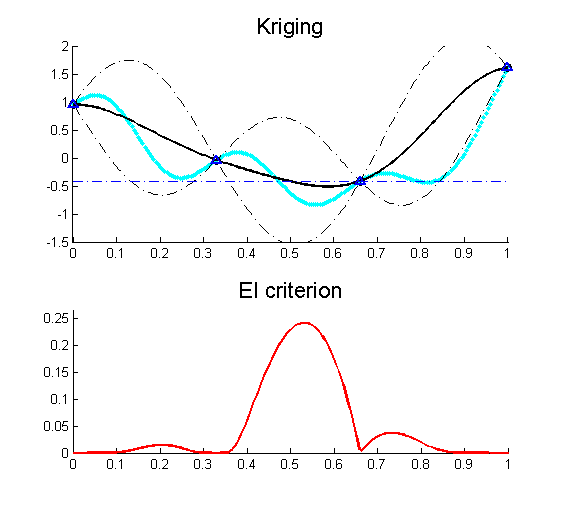
\includegraphics[width=7cm]{fig/ego1.png} \end{figure} }
%%%%%%%%%%%%%%%%%%%%%%%%%%%%%%%%%%%%%%%%%%%%%%%%%%%%%%%%%%%%%%%%%%%%%%%%%%%%%%%%%%%%%%%%%%%%%%%%%%
\frame{\frametitle{EGO: illustration  2/6}\begin{figure}[h!]  \centering	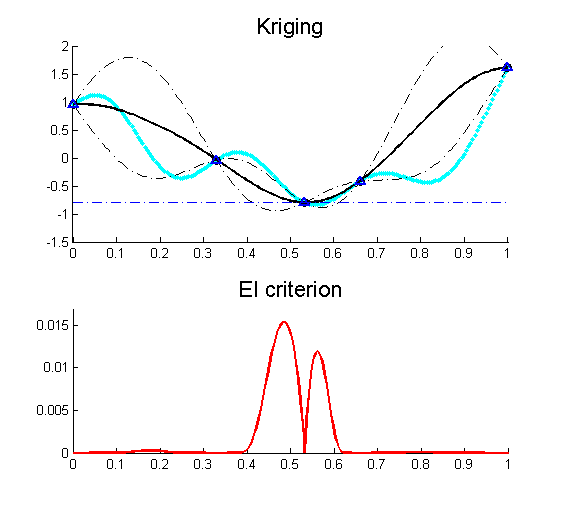
\includegraphics[width=7cm]{fig/ego2.png} \end{figure} }
%%%%%%%%%%%%%%%%%%%%%%%%%%%%%%%%%%%%%%%%%%%%%%%%%%%%%%%%%%%%%%%%%%%%%%%%%%%%%%%%%%%%%%%%%%%%%%%%%%
\frame{\frametitle{EGO: illustration  3/6}\begin{figure}[h!]  \centering	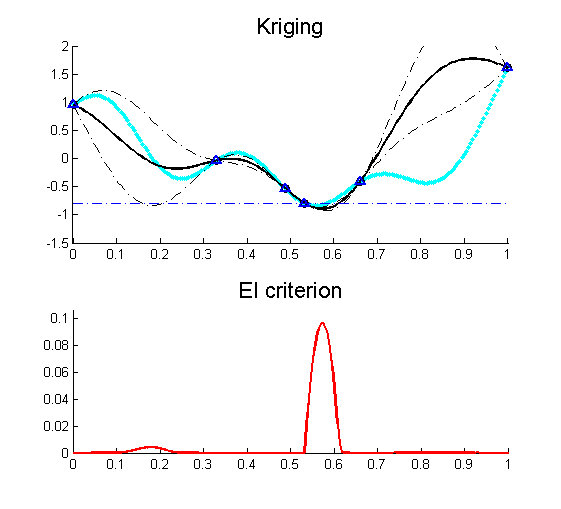
\includegraphics[width=7cm]{fig/ego3.png} \end{figure} }
%%%%%%%%%%%%%%%%%%%%%%%%%%%%%%%%%%%%%%%%%%%%%%%%%%%%%%%%%%%%%%%%%%%%%%%%%%%%%%%%%%%%%%%%%%%%%%%%%
\frame{\frametitle{EGO: illustration  4/6}\begin{figure}[h!]  \centering	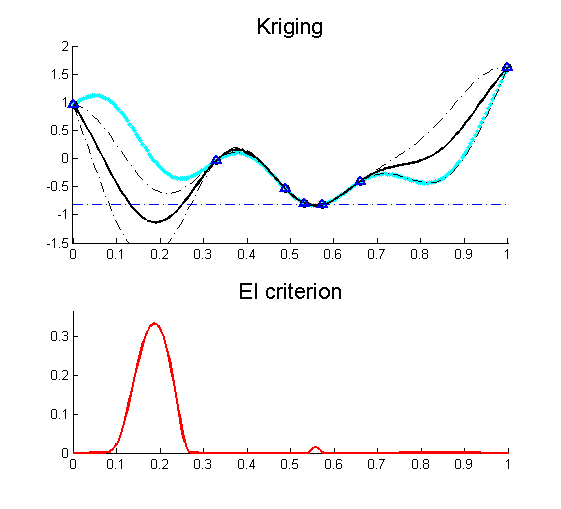
\includegraphics[width=7cm]{fig/ego4.png} \end{figure} }
%%%%%%%%%%%%%%%%%%%%%%%%%%%%%%%%%%%%%%%%%%%%%%%%%%%%%%%%%%%%%%%%%%%%%%%%%%%%%%%%%%%%%%%%%%%%%%%%%%
\frame{\frametitle{EGO: illustration  5/6}\begin{figure}[h!]  \centering	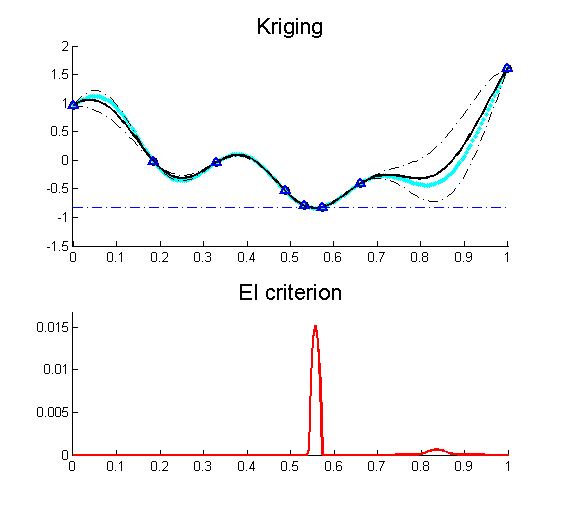
\includegraphics[width=7cm]{fig/ego5.png} \end{figure} }
%%%%%%%%%%%%%%%%%%%%%%%%%%%%%%%%%%%%%%%%%%%%%%%%%%%%%%%%%%%%%%%%%%%%%%%%%%%%%%%%%%%%%%%%%%%%%%%%%%
\frame{\frametitle{EGO: illustration  6/6}\begin{figure}[h!]  \centering	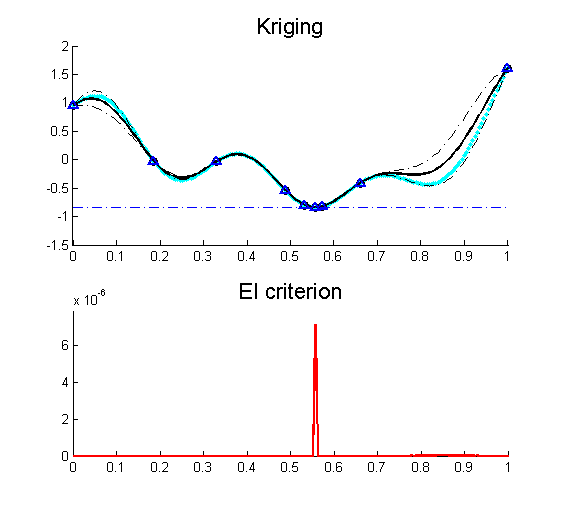
\includegraphics[width=7cm]{fig/ego6.png} \end{figure} }


%%%%%%%%%%%%%%%%%%%%%%%%%%%%%%%%%%%%%%%%%%%%%%%%%%%%%%%%%%%%%%%%%%%%%%%%%%%%%%%%%%%%%%%%%%%%%%%%%
\frame
{
\frametitle{Optimization: the noisy case}
\begin{block}{Noisy measurements}
\begin{itemize}
% \vspace{-3mm}
	\item We want to optimize: $y(\mathbf{x}_{new})$
	\item We only have access to: $\tilde y(\mathbf{x}_{new}) = y(\mathbf{x}_{new}) + \varepsilon$
\end{itemize}
\end{block}

\begin{block}{Problem with EGO}
\begin{itemize}
% \vspace{-3mm}
	\item Current minimum is unknown due to noise
	\item Future observation will also be observed in noise!
	\item $\rightarrow$ We need to rethink the notion of ``improvement''
\end{itemize}
\end{block}
}

%%%%%%%%%%%%%%%%%%%%%%%%%%%%%%%%%%%%%%%%%%%%%%%%%%%%%%%%%%%%%%%%%%%%%%%%%%%%%%%%%%%%%%%%%%%%%%%%%
\frame
{
\frametitle{Decision-making with noisy observations}
With noise, relation-order is not maintained $\rightarrow$ Which design is best?
\vspace{-3mm}
\begin{figure}[h!]  \centering	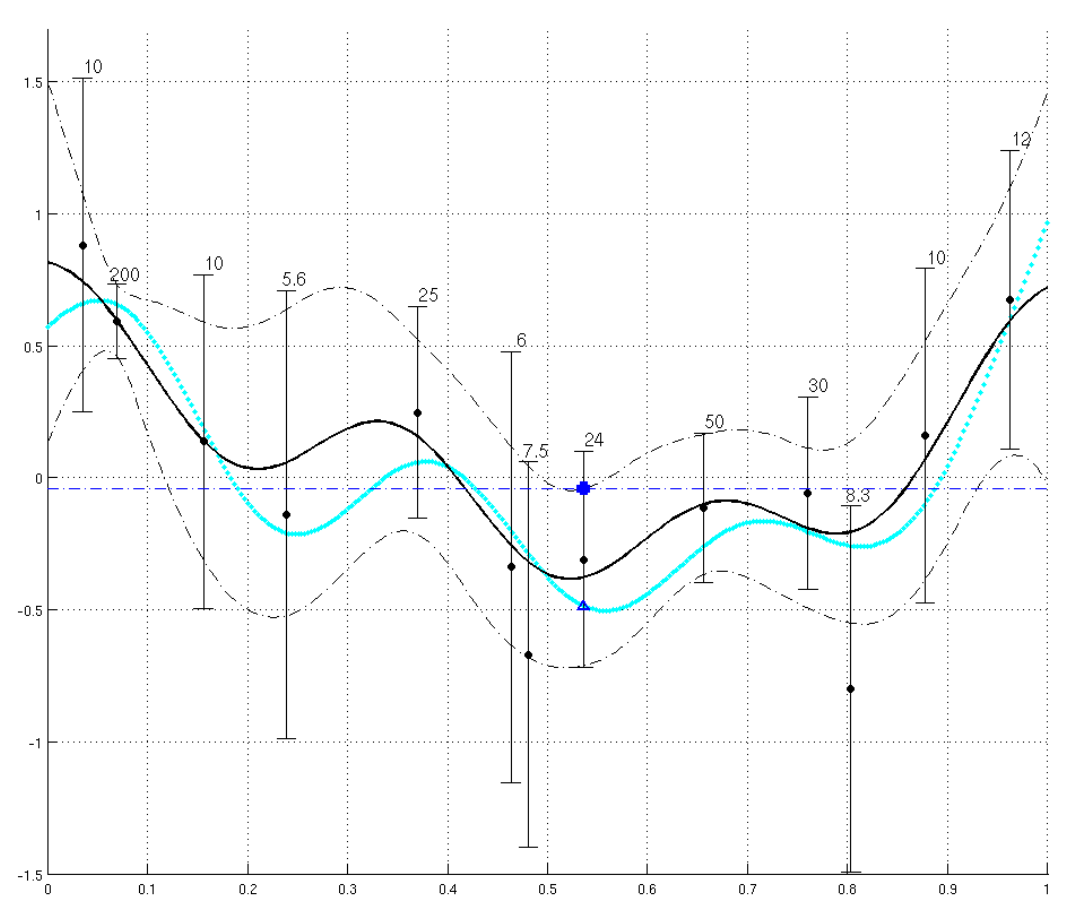
\includegraphics[width=65mm]{fig/keph.png} \end{figure}
\vspace{-4mm}
Proposition: \bf{kriging quantile}.
}

%%%%%%%%%%%%%%%%%%%%%%%%%%%%%%%%%%%%%%%%%%%%%%%%%%%%%%%%%%%%%%%%%%%%%%%%%%%%%%%%%%%%%%%%%%%%%%%%%
\frame
{
\frametitle{A criterion for noisy optimization: redefining ``improvement''}
\begin{block}{From static decision to sequential criterion}
\begin{itemize}
\vspace{-1mm}
	\item Performance: minimal kriging quantile ($q_{min}$)
	\item Improvement = gain in performance: $q_{new} - q_{min}$
\end{itemize}
\end{block}
% \vspace{-4mm}
\begin{figure}[h!]  \centering	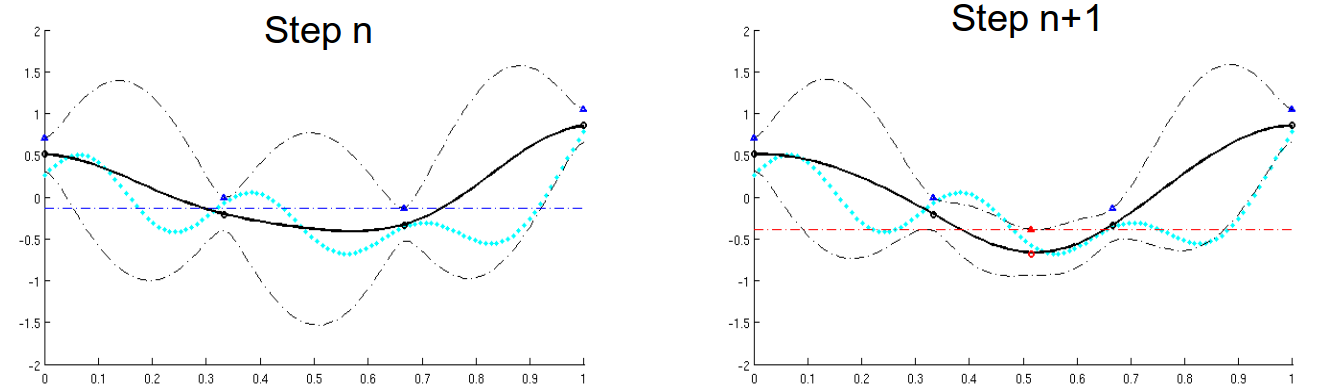
\includegraphics[width=100mm]{fig/EQIillustration.png} \end{figure}

% \begin{block}{Thanks to the analytical form of the kriging equations, EQI is analytically tractable!}
% \end{block}
}

%%%%%%%%%%%%%%%%%%%%%%%%%%%%%%%%%%%%%%%%%%%%%%%%%%%%%%%%%%%%%%%%%%%%%%%%%%%%%%%%%%%%%%%%%%%%%%%%%
\frame
{
\frametitle{Expected Quantile Improvement}
\begin{block}{Future quantile distribution}
\begin{itemize}
	\item Seen from step $n$, $Q_{n+1}$ is a Gaussian process
	\item Its moments can be calculated analytically
	\item We can measure the effect of a new measurement on the model without performing it!
\end{itemize}
\end{block}

\begin{block}{Sequential criterion}
\begin{itemize}
 \item $EQI = \mathbb{E}\left( Q_{n+1} - q_{min}  \right)$
 \item Analytically tractable
 \item Consistent with our decision criterion: one-step-look-ahead optimal strategy!
\end{itemize}

\end{block}
}

%%%%%%%%%%%%%%%%%%%%%%%%%%%%%%%%%%%%%%%%%%%%%%%%%%%%%%%%%%%%%%%%%%%%%%%%%%%%%%%%%%%%%%%%%%%%%%%%%%
\frame
{
\frametitle{EQI: illustration}
% \begin{columns}
% \begin{column}{6cm}
% 
% dfd
% 
% \end{column}
% 
% \begin{column}{4cm}
% \vspace{-0.25cm}
\begin{figure}
	\centering
		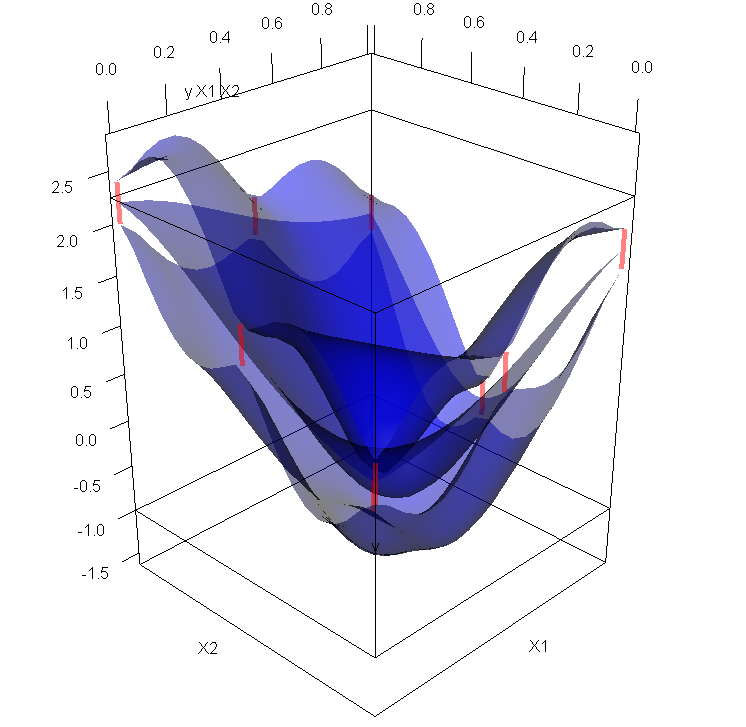
\includegraphics[width=55mm]{fig/krig.png}
% 	\label{fig:krig}
% \end{figure}
% % \vspace{-0.75cm}
% \begin{figure}
% 	\centering
		\includegraphics[width=45mm]{fig/EQI.png}
% 	\label{fig:EQI}
\end{figure}
% 
% \end{column}
% \end{columns}
}


%%%%%%%%%%%%%%%%%%%%%%%%%%%%%%%%%%%%%%%%%%%%%%%%%%%%%%%%%%%%%%%%%%%%%%%%%%%%%%%%%%%%%%%%%%%%%%%%%
\frame
{
\frametitle{Developments}
\begin{block}{Optimization strategies}
\begin{itemize}
	\item EGO-like algorithm based on EQI
	\item Specific developments (on-line allocation, cf. BIA seminar, May 2012)
\end{itemize}
\end{block}

\begin{block}{On-going and future work}
\begin{itemize}
    \item R package: \textit{DiceOptim}
    \item Adaptation to other frameworks
\end{itemize}
\end{block}
}

%%%%%%%%%%%%%%%%%%%%%%%%%%%%%%%%%%%%%%%%%%%%%%%%%%%%%%%%%%%%%%%%%%%%%%%%%%%%%%%%%%%%%%%%%%%%%%%%%
%%%%%%%%%%%%%%%%%%%%%%%%%%%%%%%%%%%%%%%%%%%%%%%%%%%%%%%%%%%%%%%%%%%%%%%%%%%%%%%%%%%%%%%%%%%%%%%%%
\section{Optimization under partial convergence}
%%%%%%%%%%%%%%%%%%%%%%%%%%%%%%%%%%%%%%%%%%%%%%%%%%%%%%%%%%%%%%%%%%%%%%%%%%%%%%%%%%%%%%%%%%%%%%%%%
%%%%%%%%%%%%%%%%%%%%%%%%%%%%%%%%%%%%%%%%%%%%%%%%%%%%%%%%%%%%%%%%%%%%%%%%%%%%%%%%%%%%%%%%%%%%%%%%%

\frame
{
\frametitle{Partial convergence: slightly opening the black-box}

\begin{block}{Partially converged simulations}
\begin{itemize}
 \item For a CFD or FEM code : internal solver (Newton-Raphson...)
 \item Idea : stop calculations before convergence
 \item Main advantage: faster response
 \item Main issue: high, auto-correlated error
\end{itemize}

\begin{block}{Objectives}
\begin{enumerate}
 \item Modeling: adapt the Gaussian process model to this framework
 \item Optimization: propose an efficient global algorithmic scheme
\end{enumerate}
\end{block}

\end{block}
}

\frame
{
\frametitle{A motivating example : 2D CFD pipe flow}
\begin{itemize}
 \item Optimization problem, 13 shape parameters
 \item OpenFOAM model : converges in 500 steps
 \item Objective function : flow SD
\end{itemize}

\vspace{-1cm}
\begin{figure}[h!]
	\centering
% 	\hspace{+0.1cm} \includegraphics[width=3cm,height=5cm]{fig/xp50reduced.png}
% 	\hspace{0.5cm} \includegraphics[width=2.8cm,height=5cm]{fig/xp2.png}
	%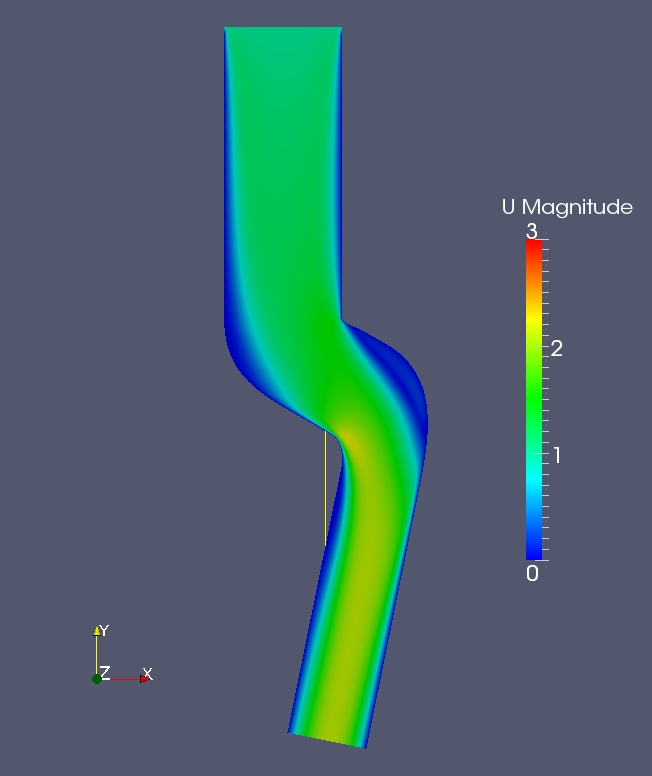
\includegraphics[width=4cm]{fig/xp_50.png}
	\hspace{1cm} 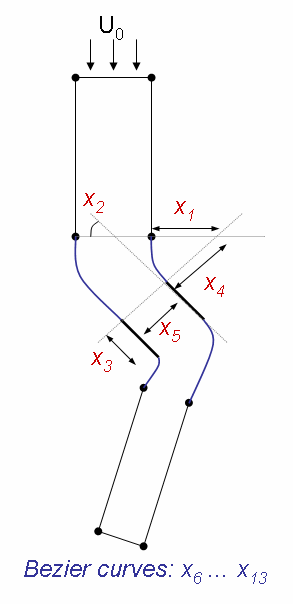
\includegraphics[width=3cm]{fig/pipeparam.png}
\end{figure}
}
%%%%%%%%%%%%%%%%%%%%%%%%%%%%%%%%%%%%%%%%%%%%%%%%%%%%%%%%%%%%%%%%%%%%%%%%%%%%%%%%%%%%%%%%%%%%%%%%%
\frame
{
\frametitle{Convergence of objective function of 20 designs}
Data: 20 LHS
\begin{figure}[htbp]
	\centering
		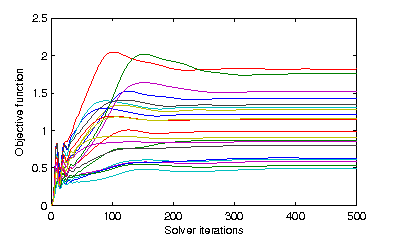
\includegraphics[width=7cm]{fig/conv20designs.png}
\end{figure}
\vspace{-5mm}
\begin{itemize}
 \item All the curves have the same shape!
 \item Information seems to be sufficient at early stage
\end{itemize}
}
%%%%%%%%%%%%%%%%%%%%%%%%%%%%%%%%%%%%%%%%%%%%%%%%%%%%%%%%%%%%%%%%%%%%%%%%%%%%%%%%%%%%%%%%%%%%%%%%%
\frame
{
\frametitle{One parameter + time analysis}
\begin{itemize}
 \item Only $x_2$ varies (most influent parameter)
 \item Analysis of 30 designs
 \item Response shows strong regularity in both design and time directions
 \item Error tends to zero
\end{itemize}
\vspace{-5mm}
\begin{figure}[h!]
	\centering
	\hspace{-1.2cm}	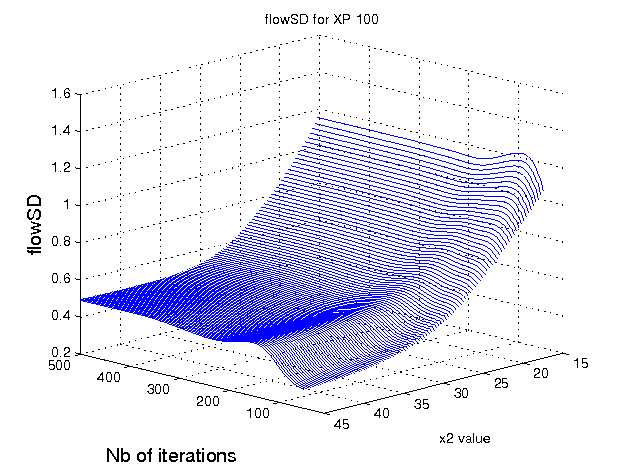
\includegraphics[width=5cm]{fig/fSD_vs_x2_and_T.png}
	            	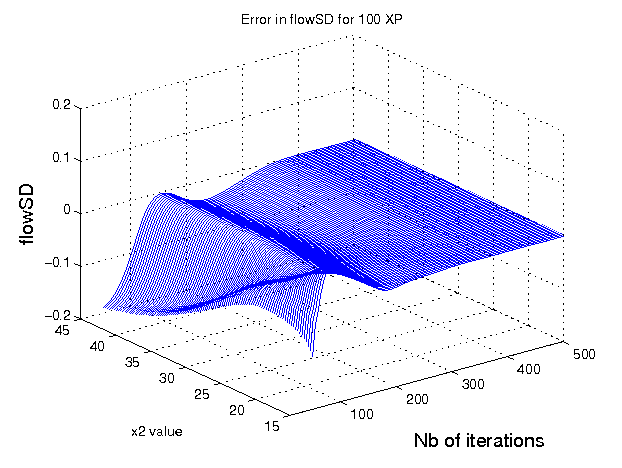
\includegraphics[width=5cm]{fig/eps_fSD_vs_x2_and_T.png}
\end{figure}
}
%%%%%%%%%%%%%%%%%%%%%%%%%%%%%%%%%%%%%%%%%%%%%%%%%%%%%%%%%%%%%%%%%%%%%%%%%%%%%%%%%%%%%%%%%%%%%%%%%
\frame
{
\frametitle{Building metamodels on partially converged data}

\begin{block}{Key features of partially converged data}
\begin{itemize}
 \item Error decreases towards zero with computational time
 \item Errors are correlated in time and design directions
 \item Error smoothness increases with time
\end{itemize}
\end{block}

\begin{block}{Proposition: build model in the joint time-design space}
\end{block}

\begin{block}{\textcolor{red}{Gaussian process paradigm $\rightarrow$ we only need to build an appropriate covariance function}}
\end{block}
}

%%%%%%%%%%%%%%%%%%%%%%%%%%%%%%%%%%%%%%%%%%%%%%%%%%%%%%%%%%%%%%%%%%%%%%%%%%%%%%%%%%%%%%%%%%%%%%%%%%
\frame
{
\frametitle{Gaussian process and partial convergence}
\begin{block}{Partially converged response = true response + error process}
$$Y(x,t) = F(x) + G(x,t)$$
with: $t$ time and $x$ design
\begin{itemize}
 \item $F(x)$ : true response - usual kriging assumptions
 \item $G(x,t)$ : error - complex structure
\end{itemize}
\end{block}

\begin{block}{Covariance function}
\begin{itemize}
	\item $k_Y(x,x',t,t') = k_F(x,x') + k_G(x,x',t,t')$
	\item $k_F$: classical stationary covariance, for instance: $k_F(x,x') = \sigma^2 exp \left( -\frac{\left\| x - x' \right\|}{\theta} \right)$
	\item $k_G$ needs to be defined
\end{itemize}
\end{block}
}

%%%%%%%%%%%%%%%%%%%%%%%%%%%%%%%%%%%%%%%%%%%%%%%%%%%%%%%%%%%%%%%%%%%%%%%%%%%%%%%%%%%%%%%%%%%%%%%%%%
\frame
{
\frametitle{Covariance of the error process}
\begin{block}{Correlation in $t$ and $x$ directions, variance decreases with $t$}
General form:
$$k_G(x,x',t,t') = \sigma^2(t,t') r_x(x, x') r_t(t, t')$$

\begin{itemize}
 \item $r_x, r_t$ : classical stationary covariances
 \item $\sigma^2(t,t')$ : decreasing function of $t$ and $t'$, for instance:
$$\sigma^2(t,t') = \sigma_G^2 \exp(- \alpha \frac{t+t'}{2})$$
\end{itemize}
\end{block}
}
%%%%%%%%%%%%%%%%%%%%%%%%%%%%%%%%%%%%%%%%%%%%%%%%%%%%%%%%%%%%%%%%%%%%%%%%%%%%%%%%%%%%%%%%%%%%%%%%%%
\frame
{
\frametitle{Final model}
\begin{block}{$Y$ is an (instationary) Gaussian process, kriging equations hold}
\begin{itemize}
 \item For any pair $u^*=[x,t]$, we have a best predictor $m(u^*)$ and prediction variance $s^2(u^*)$
 \item Prediction of converged response: $t = + \infty$
\end{itemize}
\end{block}

\begin{block}{All the response structure is contained in the covariance function $k_Y(x,x',t,t')$}
\end{block}
}
%%%%%%%%%%%%%%%%%%%%%%%%%%%%%%%%%%%%%%%%%%%%%%%%%%%%%%%%%%%%%%%%%%%%%%%%%%%%%%%%%%%%%%%%%%%%%%%%%%
\frame
{
\frametitle{Illustration}
Model for the 2D problem based on 5 runs
\begin{figure}[h!]
	\centering
		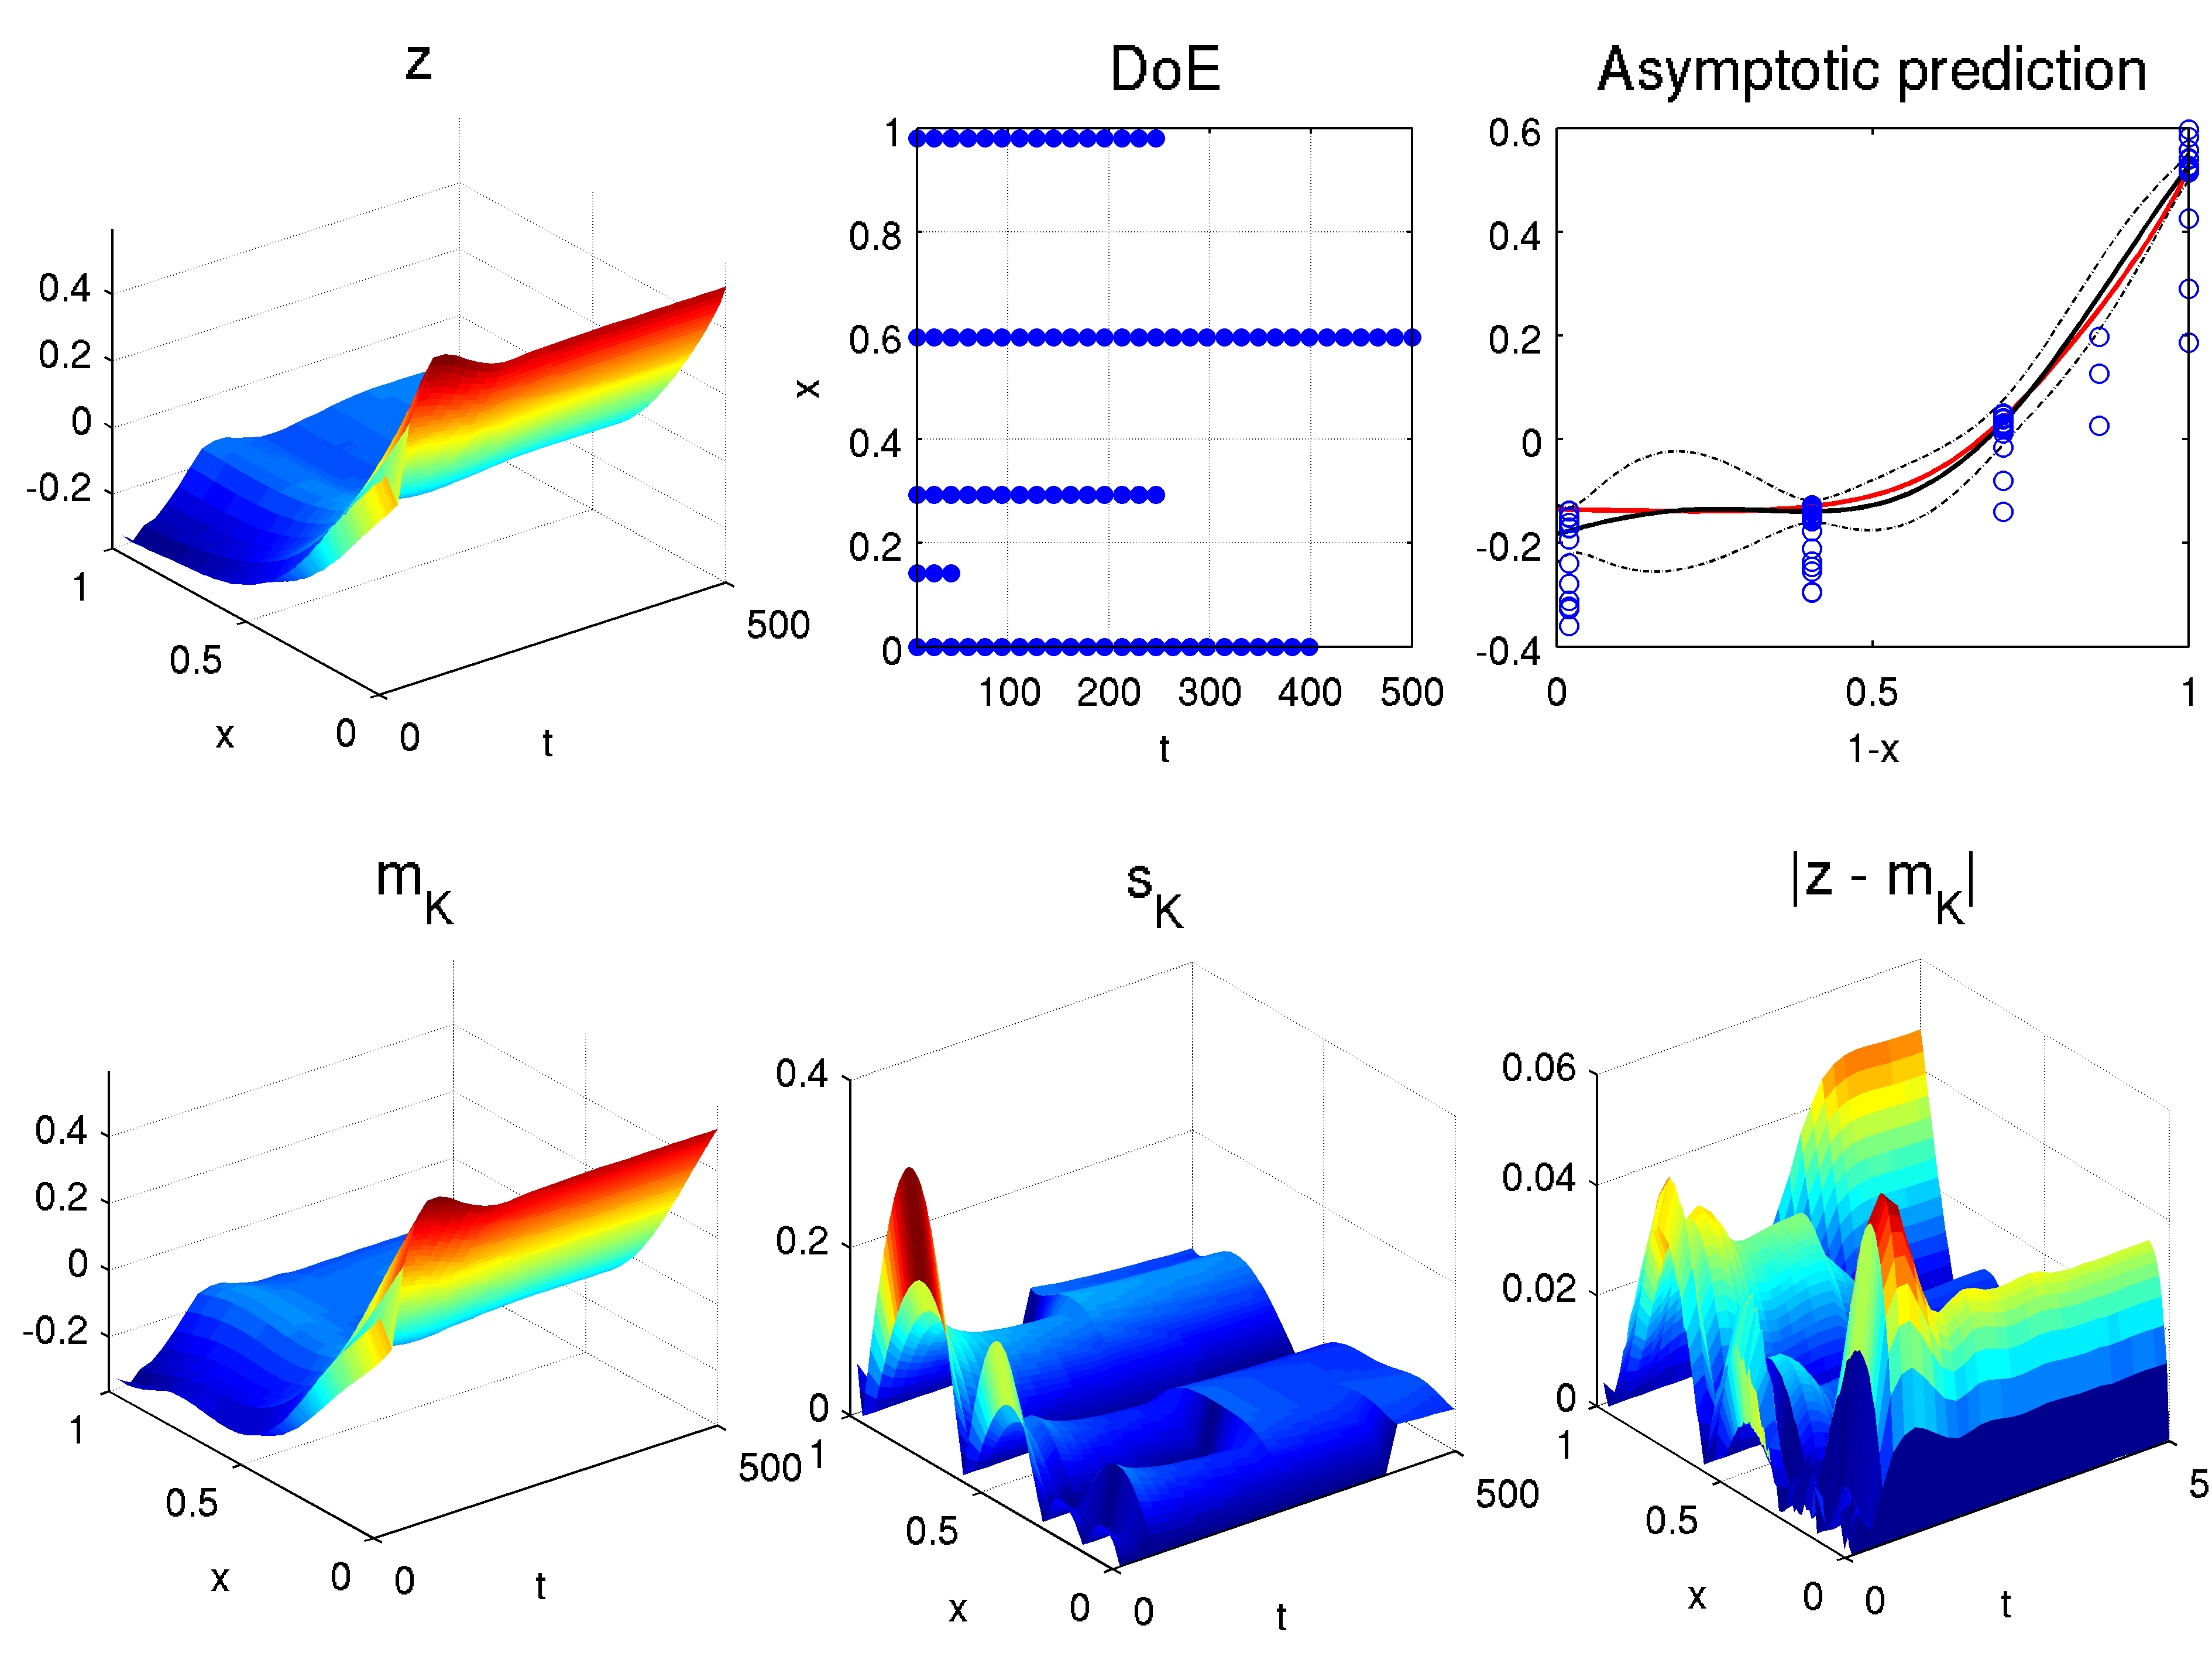
\includegraphics[width=8cm]{fig/spacetime.png}
\end{figure}
}

%%%%%%%%%%%%%%%%%%%%%%%%%%%%%%%%%%%%%%%%%%%%%%%%%%%%%%%%%%%%%%%%%%%%%%%%%%%%%%%%%%%%%%%%%%%%%%%%%%
\frame
{
\frametitle{Optimization}
\begin{block}{General framework: close to noisy optimization}
\begin{itemize}
 \item Optimize $F(x)$ when only $F(x) + G(x,t)$ is observable
 \item The Expected Quantile Improvement (EQI) idea: measure the benefit of a candidate measurement by its impact on the model
 \item Fully applicable to our framework: we measure the impact at $t=+\infty$
\end{itemize}
\end{block}

\begin{block}{Open question}
How should we choose the time $t$ invested at each measurement?
\end{block}
}

%%%%%%%%%%%%%%%%%%%%%%%%%%%%%%%%%%%%%%%%%%%%%%%%%%%%%%%%%%%%%%%%%%%%%%%%%%%%%%%%%%%%%%%%%%%%%%%%%%
\frame
{
\frametitle{Application to a toy problem}
\begin{columns}
\begin{column}{5cm}
\centering
Objective function: Branin-Hoo (2D)
\begin{figure}[h!]
	\centering
	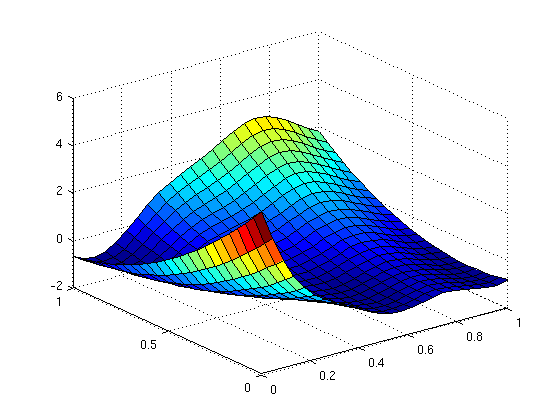
\includegraphics[width=5cm]{fig/branin2.png}
  \end{figure}
\end{column}

\begin{column}{5cm}
\centering
Error function: attenuated Hartman (3D)
  \begin{figure}[h!]
	\centering
	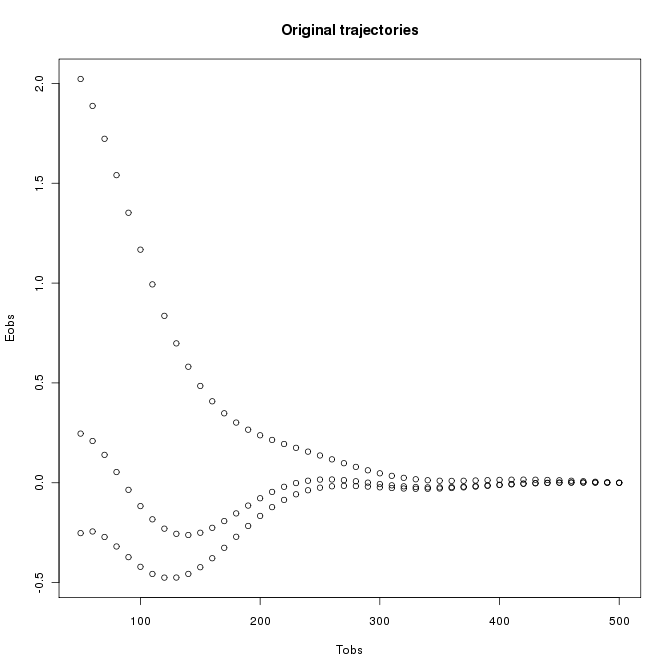
\includegraphics[width=3.5cm]{fig/3errortraj.png}
  \end{figure}
%  \end{center}
  \end{column}
\end{columns}
\begin{itemize}
 \item Full convergence: 500 time steps
 \item Initial design: 15 observations, total 3,000 steps
 \item Total budget: 8,000 steps = 16 fully converged observations
 \item At each iteration: 50 time steps allocated
\end{itemize}
}

%%%%%%%%%%%%%%%%%%%%%%%%%%%%%%%%%%%%%%%%%%%%%%%%%%%%%%%%%%%%%%%%%%%%%%%%%%%%%%%%%%%%%%%%%%%%%%%%%%
\frame
{
\frametitle{Initial stage}
\begin{figure}[h!] \centering 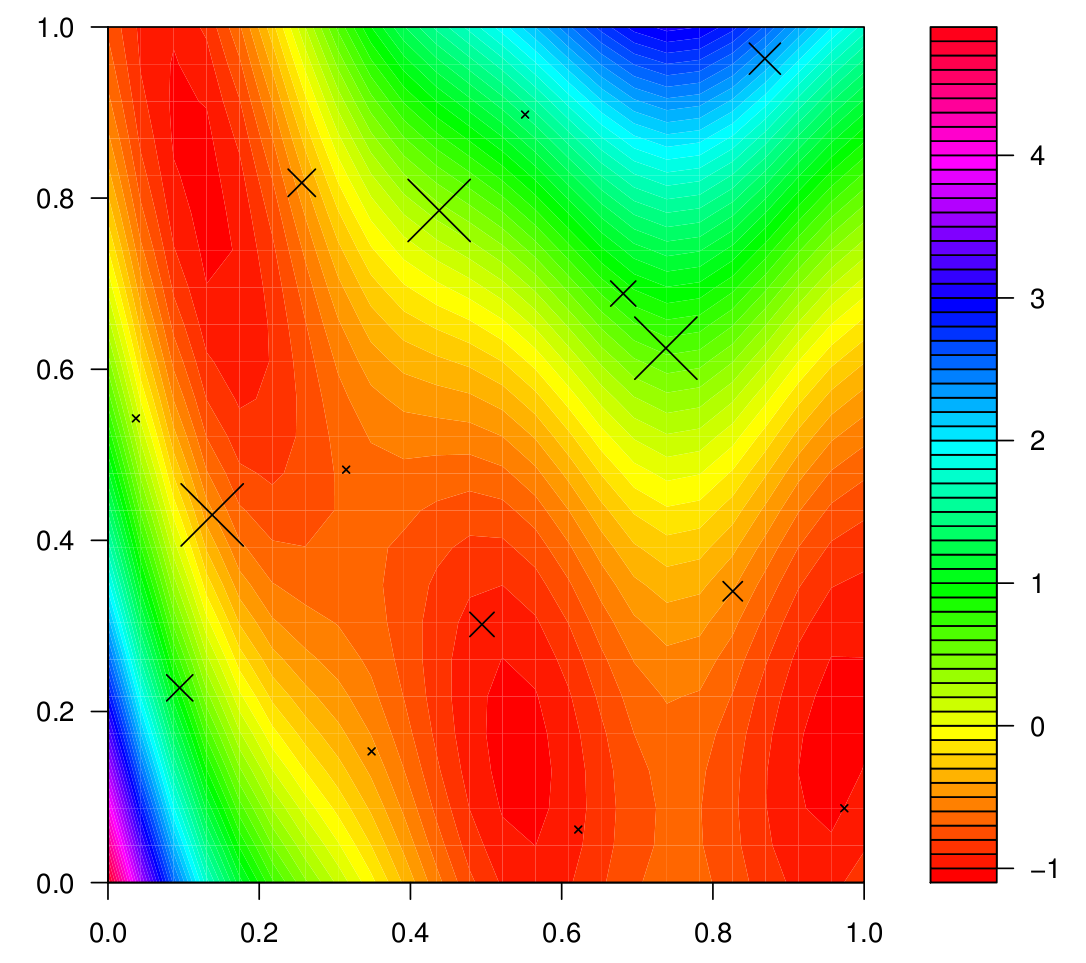
\includegraphics[width=6cm]{fig/initialBranin.png}\end{figure}
}
%%%%%%%%%%%%%%%%%%%%%%%%%%%%%%%%%%%%%%%%%%%%%%%%%%%%%%%%%%%%%%%%%%%%%%%%%%%%%%%%%%%%%%%%%%%%%%%%%%
\frame
{\frametitle{Initial stage}
\begin{figure}[h!] \centering \vspace{-3mm} 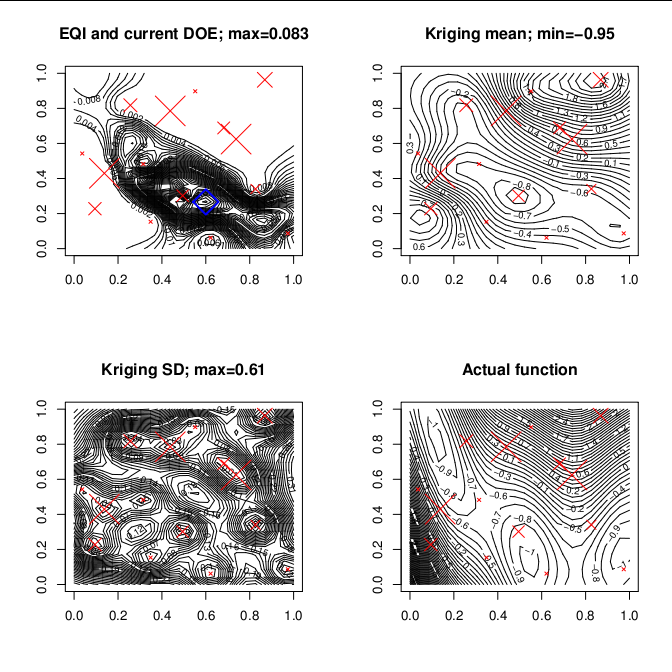
\includegraphics[trim = 10mm 17mm 10mm 9mm,clip, width=68mm]{fig/step1.png}\end{figure}}
%%%%%%%%%%%%%%%%%%%%%%%%%%%%%%%%%%%%%%%%%%%%%%%%%%%%%%%%%%%%%%%%%%%%%%%%%%%%%%%%%%%%%%%%%%%%%%%%%%
\frame
{\frametitle{After 10 iterations}
\begin{figure}[h!] \centering \vspace{-3mm} 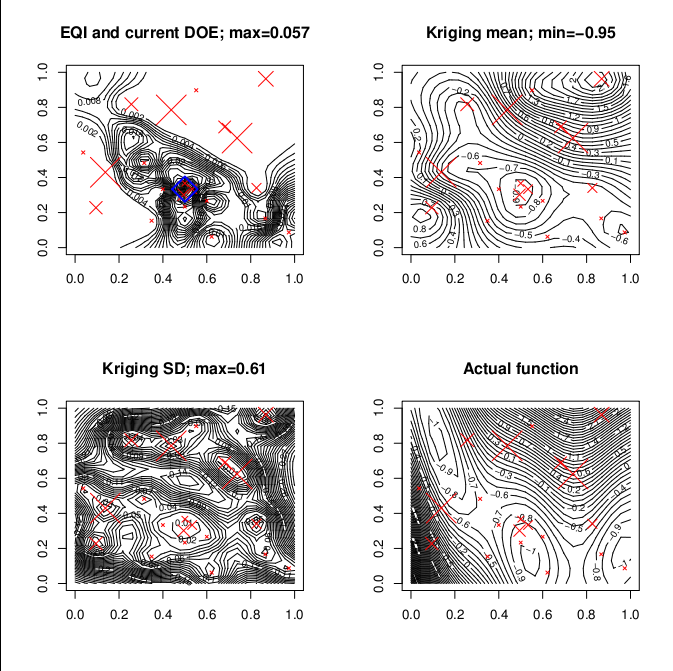
\includegraphics[trim = 10mm 17mm 10mm 9mm,clip, width=68mm]{fig/step10.png}\end{figure}}
%%%%%%%%%%%%%%%%%%%%%%%%%%%%%%%%%%%%%%%%%%%%%%%%%%%%%%%%%%%%%%%%%%%%%%%%%%%%%%%%%%%%%%%%%%%%%%%%%%
\frame
{\frametitle{After 50 iterations}
\begin{figure}[h!] \centering \vspace{-3mm} 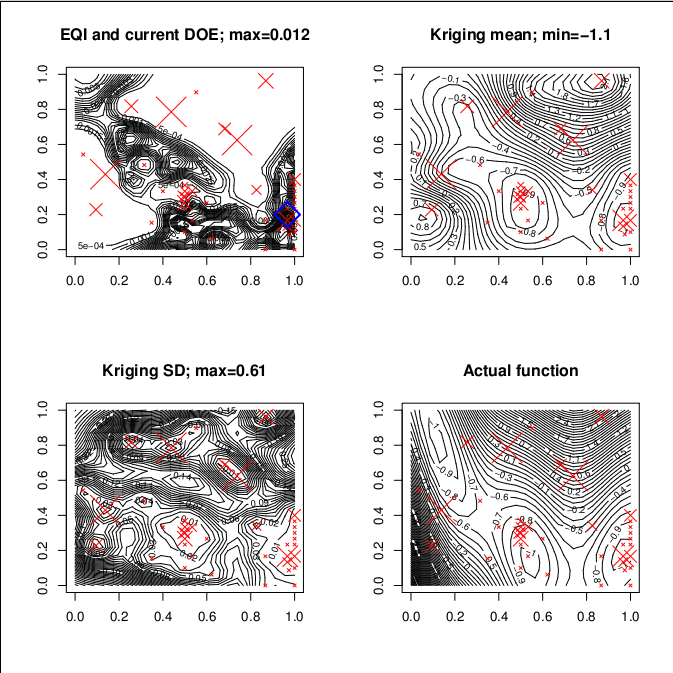
\includegraphics[trim = 10mm 17mm 10mm 9mm,clip, width=68mm]{fig/step50.png}\end{figure}}
%%%%%%%%%%%%%%%%%%%%%%%%%%%%%%%%%%%%%%%%%%%%%%%%%%%%%%%%%%%%%%%%%%%%%%%%%%%%%%%%%%%%%%%%%%%%%%%%%%
\frame
{\frametitle{After 100 iterations (final)}
\begin{figure}[h!] \centering \vspace{-3mm} 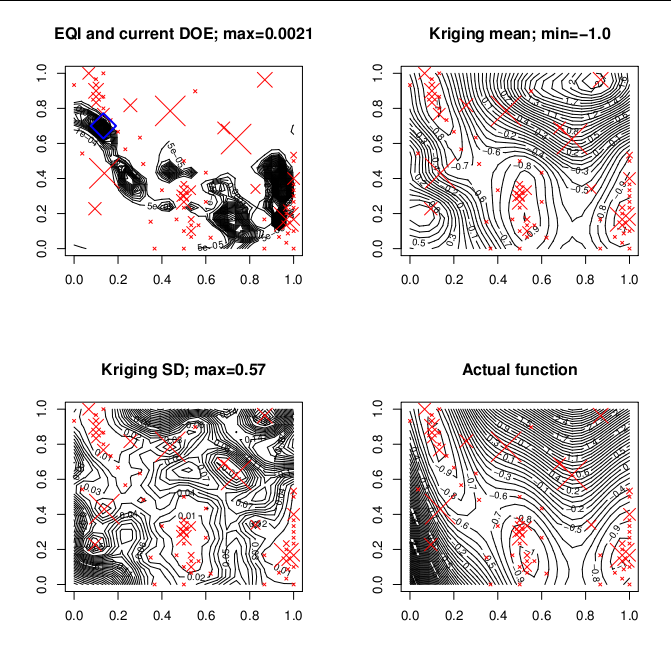
\includegraphics[trim = 10mm 17mm 10mm 9mm,clip, width=68mm]{fig/step100.png}\end{figure}}
%%%%%%%%%%%%%%%%%%%%%%%%%%%%%%%%%%%%%%%%%%%%%%%%%%%%%%%%%%%%%%%%%%%%%%%%%%%%%%%%%%%%%%%%%%%%%%%%%%
\frame
{\frametitle{Final stage}
\begin{figure}[h!] \centering 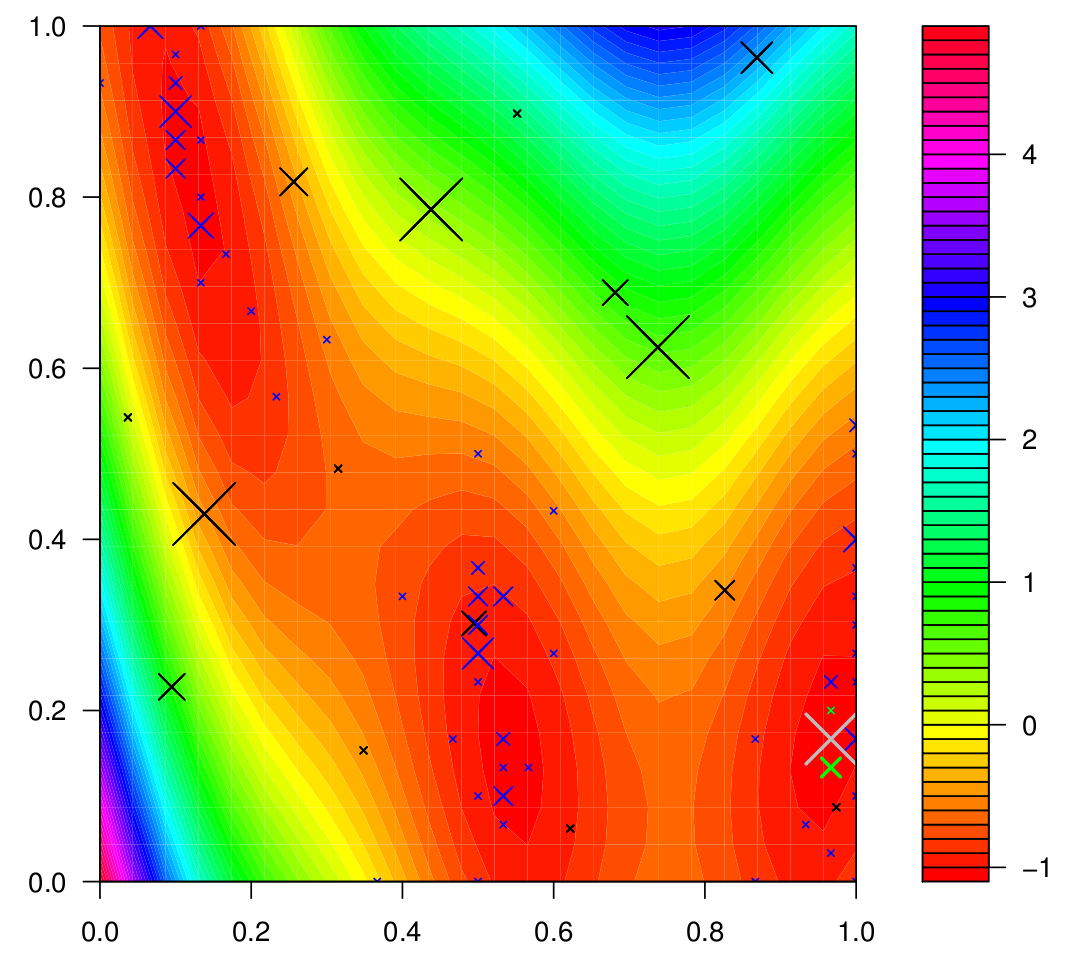
\includegraphics[width=6cm]{fig/finalBranin.png} \end{figure}}
%%%%%%%%%%%%%%%%%%%%%%%%%%%%%%%%%%%%%%%%%%%%%%%%%%%%%%%%%%%%%%%%%%%%%%%%%%%%%%%%%%%%%%%%%%%%%%%%%%
\frame
{
\frametitle{Concluding comments}

\begin{block}{Optimization under partial convergence}
\vspace{-2mm}
\begin{itemize}
 \item Many potential advantages
 \item Challenging!
\end{itemize}
\end{block}
\vspace{-2mm}
\begin{block}{Proposed solutions}
\vspace{-2mm}
\begin{itemize}
 \item Modeling: tailored Gaussian process emulator in the joint design-time space
 \item Optimisation: adaptation of the EGO algorithm
\end{itemize}
\end{block}
\vspace{-2mm}
\begin{block}{Next steps / open questions}
\vspace{-2mm}
\begin{itemize}
 \item Implementation
 \item Improvements / simplifications for a real case problem (main challenge: interface)
 \item Theoretical Developments: high dimension
\end{itemize}
\end{block}
}

%%%%%%%%%%%%%%%%%%%%%%%%%%%%%%%%%%%%%%%%%%%%%%%%%%%%%%%%%%%%%%%%%%%%%%%%%%%%%%%%%%%%%%%%%%%%%%%%
\section*{Conclusion}
%%%%%%%%%%%%%%%%%%%%%%%%%%%%%%%%%%%%%%%%%%%%%%%%%%%%%%%%%%%%%%%%%%%%%%%%%%%%%%%%%%%%%%%%%%%%%%%%

\frame
{
\frametitle{Conclusion}
\begin{block}{Gaussian process models}
\begin{itemize}
 \item Provide a lot of information
 \item Powerful tool for efficient exploitation of simulators
 \item Applicable to many frameworks / problems
\end{itemize}
\end{block}

\begin{block}{Perspectives}
\begin{itemize}
 \item Application to other frameworks
 \item Transfer of strategies to other (probabilistic) models
 \item Transfer of concepts (e.g. impact of future measurements on model)
 \item Case studies (R packages!)
\end{itemize}
\end{block}
}

\frame
{
\frametitle{References}

\footnotesize
\begin{itemize}
 \item \textit{Adaptive designs of experiments for accurate approximation of a target region}, V. Picheny, D. Ginsbourger, O. Roustant, R.T. Haftka, “”, J. Mech. Des. - July 2010 - Volume 132, Issue 7
 \item \textit{Quantile-based optimization of noisy computer experiments with tunable precision} + discussion, V. Picheny, D. Ginsbourger, Y. Richet, G. Caplin, Technometrics, 2013
 \item \textit{Approximating computer experiments using partially converged simulations and a Gaussian process emulator}, V. Picheny, D. Ginsbourger, minor revision, 2012
 \item \textit{KrigInv: Kriging-based Inversion for Deterministic and Noisy Computer Experiments}, C. Chevalier, V. Picheny, D. Ginsbourger
 \item \textit{DiceOptim: Kriging-based optimization for computer experiments}, D. Ginsbourger, V. Picheny, O. Roustant
\end{itemize}
}


\end{document}
